\documentclass{beamer}

\usepackage[utf8]{inputenc}
\usepackage{default}
\usetheme{Singapore}
\usecolortheme{orchid}

\title{Visualising Flow Algorithms\\ \vspace{0.5cm}
Maximum Flow: Ford-Fulkerson\\
Minimum Cost Flow: Cycle Cancelling\\
}
\author{Quirin Fischer}
\date{IDP presentation\\August 8, 2016}

\usepackage{bm}
\newcommand*{\vecval}[1]{\bm{#1}}
\newcommand*{\R}{\mathbb{R}}

\begin{document}
\beamertemplatenavigationsymbolsempty

\frame{\titlepage}

\frame{
\frametitle{Previous Work}
\begin{itemize}
    \item Lots more graph algorithm visualisations 
    \begin{itemize}
        \item Shortest paths
        \item Spanning trees
        \item Matchings
        \item ...
    \end{itemize}
    \item Reusable page layout
    \item Graph visualisation code
\end{itemize}
}

\frame{
\centering
    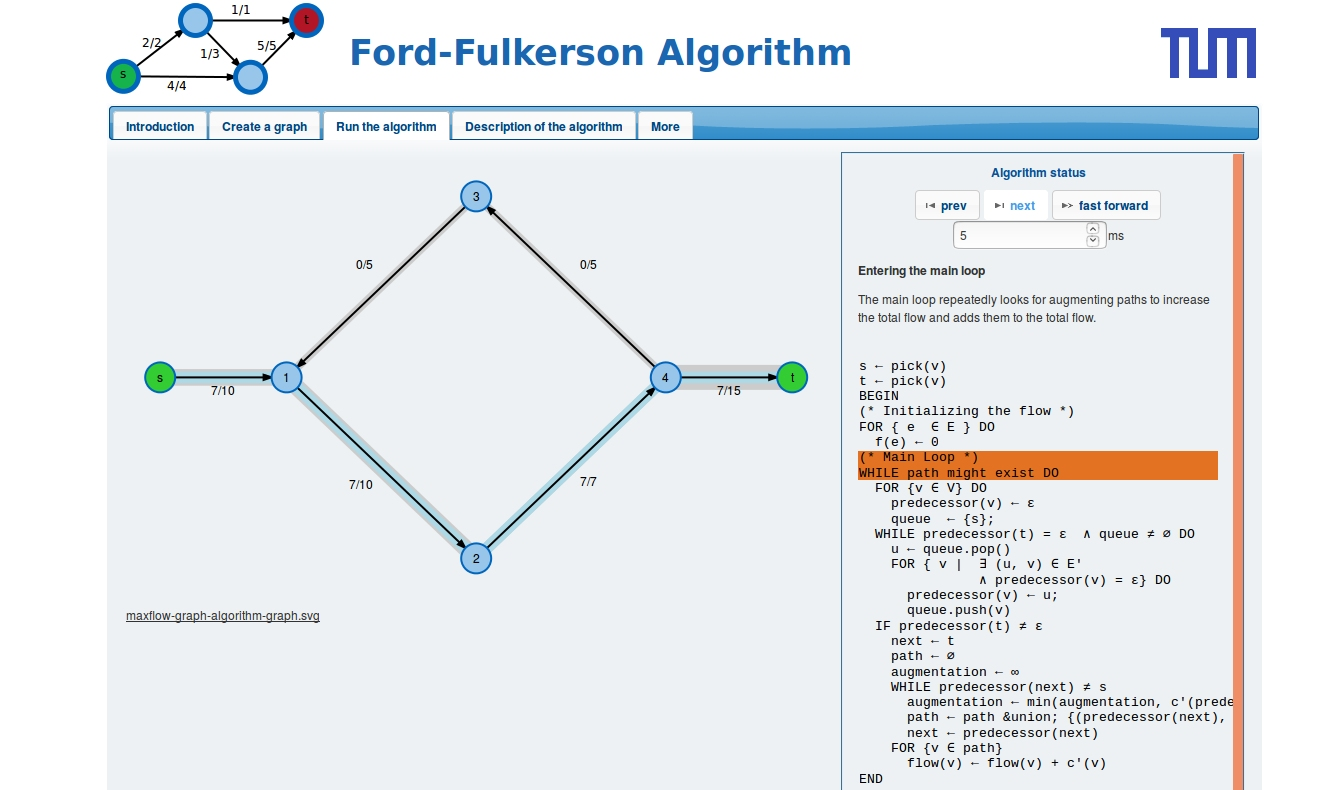
\includegraphics[width=\textwidth]{images/algorithm-example.jpg}
}

\frame{
\frametitle{Scope of the project}
\begin{itemize}
    \item Implement visualisations for flow problems
    \begin{itemize}
        \item Maximum flow: Ford-Fulkerson
        \item Minimum Cost Flow: Cycle Cancelling
    \end{itemize}
    \item Write logic for algorithms, reuse code
    \item Adapt/extend visualisation
    \item Text content
    \item Additional interactive resources 
\end{itemize}
}

\frame{
\frametitle{Flow Networks}

\begin{minipage}{0.47\textwidth}
    \begin{itemize}
        \item Directed graph $G = (V, E)$
        \item Edge capacities\\ Source and Target\\ $N = (G, c(e), s, t)$
        \item $\forall e \in E: c(e) \geq 0$
        \item $s \in V, t \in V, s\neq t$
        
    \end{itemize}
\end{minipage}
\begin{minipage}{0.5\textwidth}
\centering
    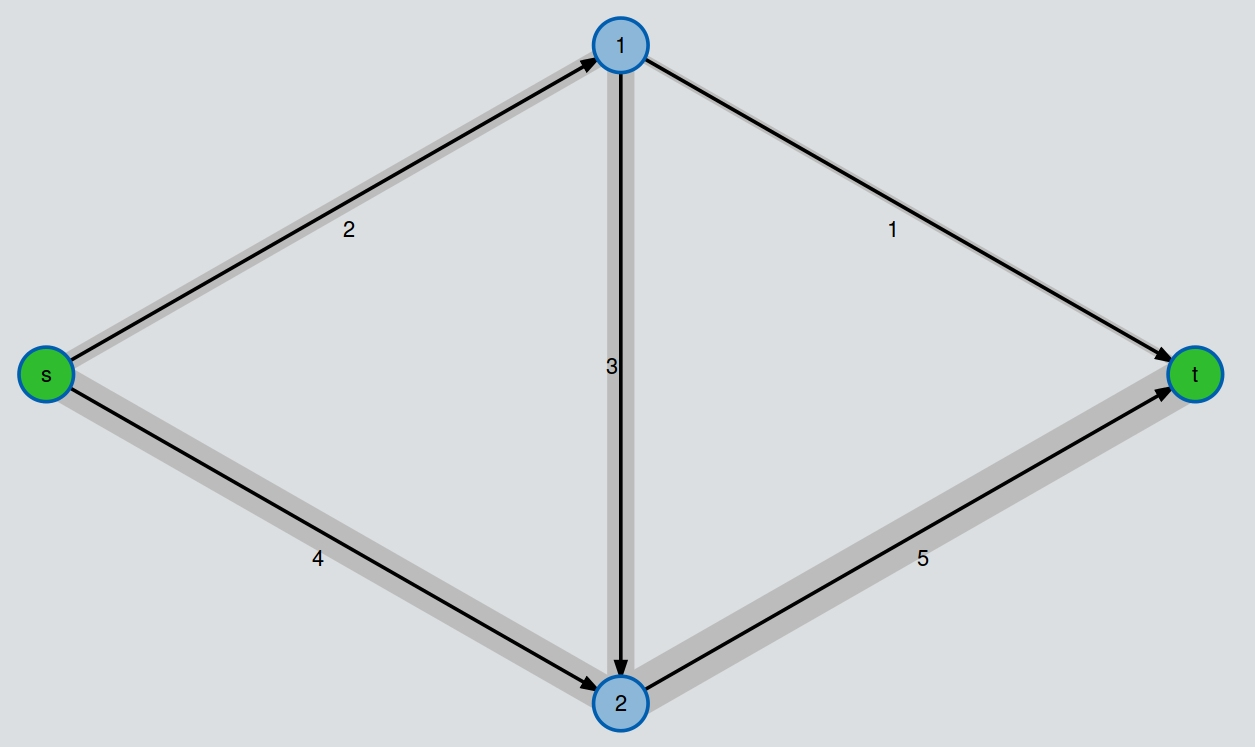
\includegraphics[width=0.9\textwidth]{images/network.jpg}
\end{minipage}
}


\frame{
\frametitle{Maximum Flow Problem}

\begin{itemize}
    \item Flow: $f(e)$
    \item Feasibility:  $\forall e \in E: 0 \leq f(e) \leq c(e)$
    \item Flow conservation:  $\forall v \in V \setminus \{s, t\}: \sum_{e: (u, v), u \in V} f(e) = \sum_{e: (v, u), u \in V} f(e)$
\end{itemize}
}

\frame{
\frametitle{Residual Graph}

\begin{minipage}{0.47\textwidth}
    \begin{itemize}
        \item Determined by flow in a network
        \item New edges, different capacities:
            \begin{itemize}
                \item Forward edges: $c'(e) = c(e) - f(e) | c'(e) > 0$
                \item Backward edges: $c'(e') = f(e) | e: (u, v), e': (v, u)$
            \end{itemize}
    \end{itemize}
\end{minipage}
\begin{minipage}{0.5\textwidth}
\centering
    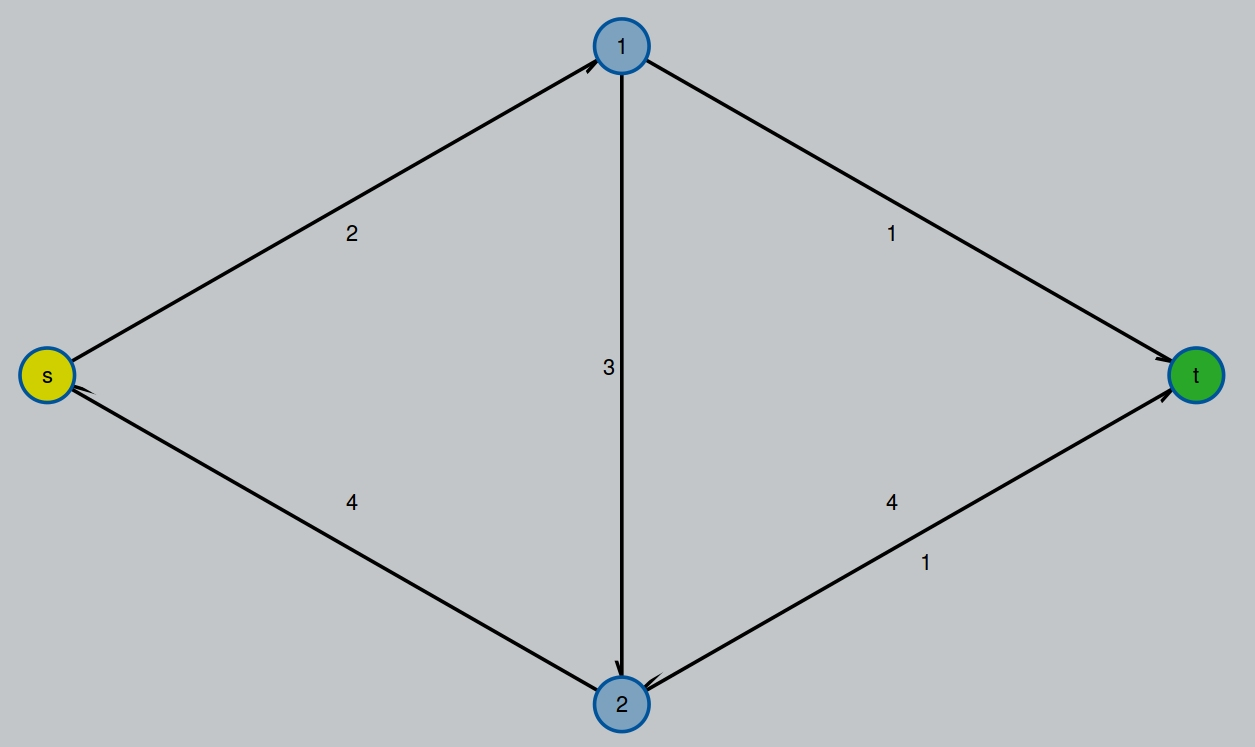
\includegraphics[width=0.9\textwidth]{images/residual.jpg}
\end{minipage}
}

\frame{
\frametitle{The Ford-Fulkerson Algorithm}

\begin{itemize}
    \item Find paths from $s$ to $t$ in the residual graph
    \item Adjust to saturate one edge
    \item Repeat until no more path exists
\end{itemize}

}

%\frame{
%visualisation
%}


\frame{
\frametitle{Minimum Cost Flow Problem}

\begin{itemize}
    \item Additional structure: edge cost $a(e)$
    \item Cost of a flow:  $\sum_{e\in E} f(e)\cdot a(e)$
    \item Fixed amount of flow
    \item Minimize cost of used edges
\end{itemize}
}

\frame{
\frametitle{Cycle-Cancelling Algorithm}

\begin{itemize}
    \item First, compute maximum flow
    \item Residual cost graph
    \item Identify negative cycles\\
        Bellman-Ford algorithm\\
        Negative cycle is signalled by target node
    \item Redirect flow along cycle
\end{itemize}

}

\frame{
\frametitle{Implementation Details}
\begin{itemize}
    \item HTML page, Javascript for animation
    \item Vector graphics for visualisation
    \item D3 to bind data to elements
\end{itemize}
}

\frame{
\frametitle{HTML}
\begin{minipage}{0.47\textwidth}
    \begin{itemize}
        \item Tab structure of the page
        \item Empty svg element for visualisation
        \item Static elements for algorithm
        \begin{itemize}
            \item Description of steps
            \item Corresponding pseudocode
            \item Static elements for algorithm
        \end{itemize}
    \end{itemize}
\end{minipage}
\begin{minipage}{0.5\textwidth}
\centering
    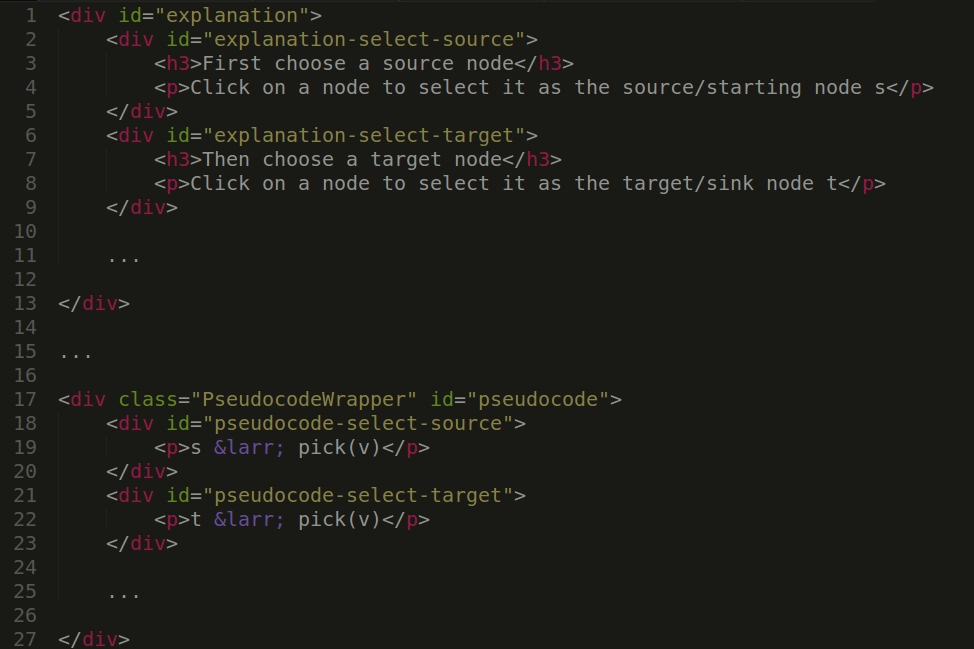
\includegraphics[width=0.9\textwidth]{images/html.jpg}
\end{minipage}
}

\frame{
\frametitle{Javascript}
\begin{minipage}{0.47\textwidth}
    \begin{itemize}
        \item Keep track of algorithm state
        \item Transition functions
        \item Existing structure for step/undo
        \item Update display
    \end{itemize}
\end{minipage}
\begin{minipage}{0.5\textwidth}
\centering
    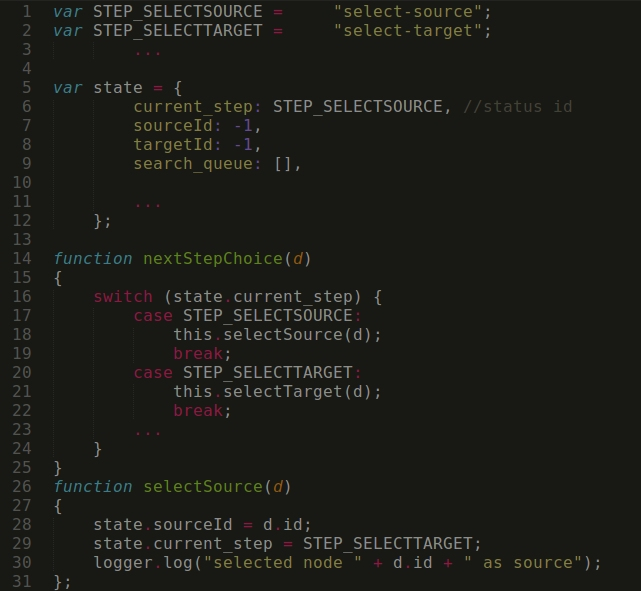
\includegraphics[width=0.9\textwidth]{images/js.jpg}
\end{minipage}
}

\frame{
\frametitle{Updating with D3}

    \begin{itemize}
        \item Set of HTML elements $H$, Data set $D$
        \item Fixed assignment: $\left(h_i, d_i\right)$
        \item HTML attributes as function of data, e.g. $h_{i, \text{stroke\_width}}= calculate\_stroke(d_i)$
        \item Update for changed data
        \item Special handlers for added and removed elements
            \begin{itemize}
                \item $\left(\epsilon, d_i\right) \rightarrow Create $ 
                \item $\left(d_i, \epsilon \right) \rightarrow Delete $ 
            \end{itemize}
    \end{itemize}

}

\frame{
\frametitle{D3 - code}

\centering
    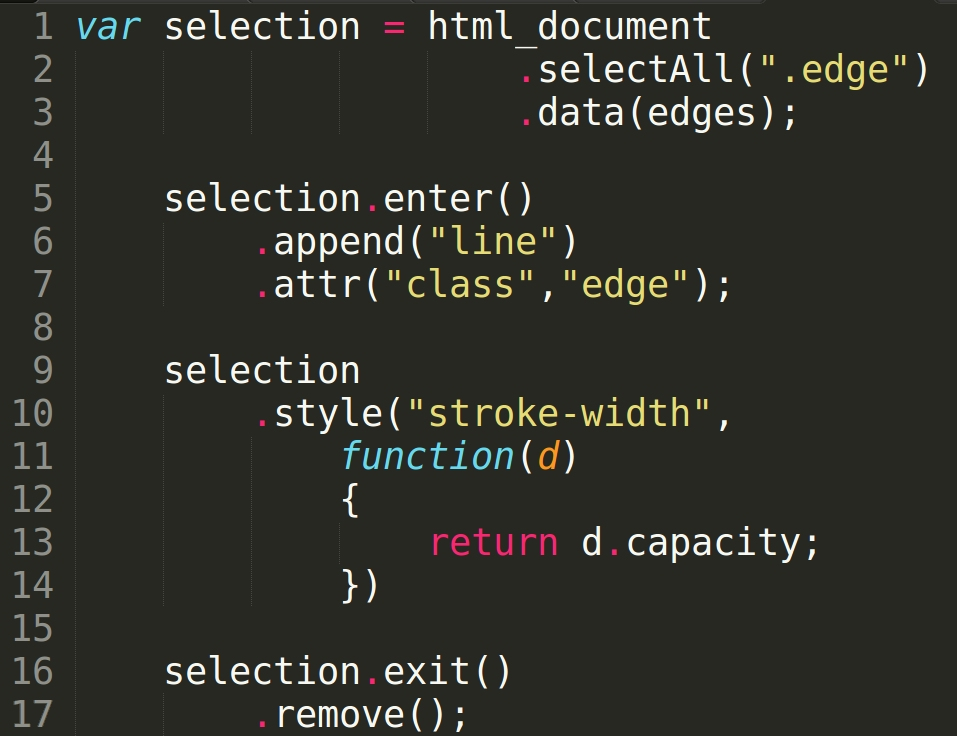
\includegraphics[width=0.6\textwidth]{images/d3.jpg}

}


\frame{
\centering
\huge{Thank you! \\ Questions?}
}
\end{document}
